\documentclass[12pt,letterpaper]{article}
\usepackage{fullpage}
\usepackage[top=2cm, bottom=4.5cm, left=2.5cm, right=2.5cm]{geometry}
\usepackage{amsmath,amsthm,amsfonts,amssymb,amscd}
\usepackage{lastpage}
\usepackage{enumerate}
\usepackage{fancyhdr}
\usepackage{mathrsfs}
\usepackage{xcolor}
\usepackage{graphicx}
\usepackage{listings}
\usepackage{hyperref}
\usepackage{graphicx}
\usepackage{tikz}

\definecolor{codegreen}{rgb}{0,0.6,0}
\definecolor{codegray}{rgb}{0.5,0.5,0.5}
\definecolor{codepurple}{rgb}{0.58,0,0.82}
\definecolor{backcolour}{rgb}{0.95,0.95,0.92}

\lstdefinestyle{mystyle}{
    backgroundcolor=\color{backcolour},   
    commentstyle=\color{codegreen},
    keywordstyle=\color{magenta},
    numberstyle=\tiny\color{codegray},
    stringstyle=\color{codepurple},
    basicstyle=\ttfamily\footnotesize,
    breakatwhitespace=false,         
    breaklines=true,                 
    captionpos=b,                    
    keepspaces=true,                 
    numbers=left,                    
    numbersep=5pt,                  
    showspaces=false,                
    showstringspaces=false,
    showtabs=false,                  
    tabsize=2
}

\lstset{style=mystyle}

\hypersetup{%
  colorlinks=true,
  linkcolor=blue,
  linkbordercolor={0 0 1}
}
 
\renewcommand\lstlistingname{Algorithm}
\renewcommand\lstlistlistingname{Algorithms}
\def\lstlistingautorefname{Alg.}

\lstdefinestyle{Python}{
    language        = Python,
    frame           = lines, 
    basicstyle      = \footnotesize,
    keywordstyle    = \color{blue},
    stringstyle     = \color{green},
    commentstyle    = \color{red}\ttfamily
}

\setlength{\parindent}{0.0in}
\setlength{\parskip}{0.05in}

% Edit these as appropriate
\newcommand\course{CSE 3500}
\newcommand\hwnumber{2}                  % <-- homework number
\newcommand\NetIDa{bec19009}           % <-- NetID of person #1

\pagestyle{fancyplain}
\headheight 35pt
\lhead{\NetIDa}
\chead{\textbf{\Large Homework \hwnumber}}
\rhead{\course \\ \today}
\lfoot{}
\cfoot{}
\rfoot{\small\thepage}
\headsep 1.5em

\begin{document}

\begin{center}
    \LARGE Divide-and-conquer problem set
\end{center}

\section*{Problem 0}

Give upper $(O(\cdot))$ asymptotic bounds for the following recurrences. You may assume a $O(1)$
base case for small $n$. Justify your answer by some combination of the following: deriving
how much total work is done at an arbitrary level $k$, how many levels there are, and how
much work is required to merge (function body). For each recurrence, state whether or not
it is top-heavy, bottom-heavy, or even work. Answers that only cite the Master theorem will
not receive full credit.

\begin{enumerate}
    \item{$T(n) = 2T(\frac{n}{2})+O(n)$}
    \item{$T(n) = 2T(\frac{n}{2})+O(1)$}
    \item{$T(n) = 7T(\frac{n}{2})+O(n^3)$}
    \item{$T(n) = 7T(\frac{n}{2})+O(n^2)$}
    \item{$T(n) = 4T(\frac{n}{2})+O(n^2\sqrt{n})$}
    \item{$T(n) = 4T(\frac{n}{2})+O(n\log_2(n))$}
\end{enumerate}

For each of the following problems, we can infer a base case when $n = 1$ then the output would be $1$.
This is because for any of these problems, if there is only one element then only that element needs to be cheked.

\begin{enumerate}
    \item We can create a equation for each level $k$ of the recusion tree by finding what each levels equation is. Our first level down 
    can be derived from what $T(\frac{n}{2})$ is equal to.
    We can do this by dividing $2T(\frac{n}{2})+n$ by 2 which gets us $2T(\frac{n}{2^2})+\frac{n}{2}$. We can then
    then plug this into the original equation of $2T(\frac{n}{2})+n$ to get $2[2T(\frac{n}{2^2}) + \frac{n}{2}] + n$ which
    simplifies to $2^2T(\frac{n}{2^2}) + 2n$. We can use this process to find what $T(\frac{n}{2^3})$ is and from that, plug that
    into the equation to get $2^3T(\frac{n}{2^3}) + 3n$. We can repeat this process until we get to $T(n) = 2^kT(\frac{n}{2^k}) + kn$
    where $k$ is the number of levels in the recursion tree. We can now also assume $T(\frac{n}{2^k})$ is trying to reach $1$ which is the base case.
    We now solve for $k$ from $T(\frac{n}{2^k}) = T(1)$ to get 
    $n = 2^k$ which gives us $k = \log_2(n)$. We can now plug this into the equation to get $T(n) = 2^{\log_2(n)}T(1) + n\log_2(n)$ which
    simplifies down to $T(n) = nT(1) + n\log(n)$ or $T(n) = O(nlog(n))$. This would have a even work distribution because as $n$ increases, the
    amount of work done at each level increases by a constant factor. We can also calculate the recurrence that is equal to 1 meaning that
    the amount of work is even.
    \item Just like the previous questions, we can create a equation for each level $k$ of the recusion tree by finding what $T(\frac{n}{2})$ is equal to.
    We can do this by dividing $2T(\frac{n}{2})+1$ by 2 which gets us $2T(\frac{n}{2^2})+\frac{1}{2}$. We can then
    then plug this into the original equation of $2T(\frac{n}{2})+1$ to get $2[2T(\frac{n}{2^2}) + \frac{1}{2}] + 1$ which
    simplifies to $2^2T(\frac{n}{2^2}) + 2$. We can repeat this process until we get to $T(n) = 2^kT(\frac{n}{2^k}) + k$
    where $k$ is the number of levels in the recursion tree. We can now also solve for $k$ from $T(\frac{n}{2^k}) = T(1)$ to get
    $n = 2^k$ which gives us $k = \log_2(n)$. We can now plug this into the equation to get $T(n) = 2^{\log_2(n)}T(1) + n$ which
    simplifies down to $T(n) = nT(1) + n$ or $T(n) = O(n)$. This is a bottom-heavy recusion because the work done at each
    level is $O(1)$ and the number of levels is $O(\log(n))$. This means that there is more work done on the bottom/last levels,
    rather than the top with the total work done being $O(n)$. We can also check to see that the recurrence relation is greater than 1
    meaning that the work done at each level is greater than the work done at the previous level.
    \item This question is similar to the previous two questions. We can create a equation for each level $k$ of the recusion tree by finding what $T(\frac{n}{2})$ is equal to.
    We can do this by dividing $7T(\frac{n}{2})+n^3$ by 2 which gets us $7T(\frac{n}{2^2})+\frac{n^3}{2}$. We can then
    then plug this into the original equation of $7T(\frac{n}{2})+n^3$ to get $7[7T(\frac{n}{2^2}) + \frac{n^3}{2}] + n^3$ which
    simplifies to $7^2T(\frac{n}{2^2}) + 7(\frac{n^3}{2}) + n^3$. We can repeat this process $k$ times until we get to $T(n) = 7^kT(\frac{n}{2^k}) + 7^{k-1}(\frac{n^3}{2^{k-1}})+ ... 7(\frac{n^3}{2}) + n^3$
    where $k$ is the number of levels in the recursion tree. We can now also solve for $k$ from $T(\frac{n}{2^k}) = T(1)$ to get 
    $n = 2^k$ which gives us $k = \log_2(n)$. We can now plug this into the equation to get $T(n) = 7^{\log(n)}T(1) + 7^{\log(n)-1}(\frac{n^3}{2^{\log(n)-1}})+ ... 7(\frac{n^3}{2}) + n^3$ which
    simplifies down to $T(n) = n^{\log_2(7)}T(1) + n^3$ or $T(n) = O(n^3)$. This is a top-heavy recusion because the work done at each
    level is $O(n^3)$ which heavily outweights $n^{\log_2(7)}$ and the number of levels is $O(\log(n))$. This means that the total work done is $O(n^3)$.
    \item This problem is similar to the previous question. We can create a equation for each level $k$ of the recusion tree by finding what $T(\frac{n}{2})$ is equal to.
    We can do the same process as the previous question by dividing by 2 then plugging it back into the original equation. For this case for $T(\frac{n}{2})$
    we get $7T(\frac{n}{2^2}) + \frac{n^2}{2}$ and once we plug this into the original equation we get $7[7T(\frac{n}{2^2}) + \frac{n^2}{2}] + n^2$ which
    simplifies to $7^2T(\frac{n}{2^2}) + 7(\frac{n^2}{2}) + n^2$. We can repeat this process $k$ times until we get to $T(n) = 7^kT(\frac{n}{2^k}) + 7^{k-1}(\frac{n^2}{2^{k-1}})+ ... 7(\frac{n^2}{2}) + n^2$
    where $k$ is the number of levels in the recursion tree. We can now also solve for $k$ from $T(\frac{n}{2^k}) = T(1)$ to get 
    $n = 2^k$ which gives us $k = \log_2(n)$. We can now plug this into the equation to get $T(n) = 7^{\log(n)}T(1) + 7^{\log(n)-1}(\frac{n^2}{2^{\log(n)-1}})+ ... 7(\frac{n^2}{2}) + n^2$ which
    simplifies down to $T(n) = n^{\log_2(7)}T(1) + n^2$. If we solve out $n^{\log_2(7)}$ we get $n^{2.81}$ which grows faster than $n^2$ so we can say that this is exactly
    $T(n) = O(n^{\log_2(7)})$. This is a bottom-heavy recusion because the work done as $O(n^{\log_2(7)})$ overweighs
    $n^2$ at higher levels making the total work done $O(n^{\log_2(7)})$.
    \item Like all the previous questions, we can create a equation for each level $k$ of the recusion tree by finding what $T(\frac{n}{2})$ is equal to.
    We first divide $4T(\frac{n}{2})+n^2\sqrt{n}$ by 2 to get $4T(\frac{n}{2^2}) + \frac{n^2\sqrt{n}}{2}$. 
    We can then plug this into the original equation of $4T(\frac{n}{2})+n^2\sqrt{n}$ to get $4[4T(\frac{n}{2^2}) + \frac{n^2\sqrt{n}}{2}] + n^2\sqrt{n}$ which
    simplifies to $4^2T(\frac{n}{2^2}) + 3n^2\sqrt{n}$. We can repeat this process $k$ times until we get to $T(n) = 4^kT(\frac{n}{2^k}) + (2^k-1)n^2\sqrt{n}$.
    We can now also solve for $k$ from $T(\frac{n}{2^k}) = T(1)$ to get $n = 2^k$ which gives us $k = \log_2(n)$. We can now plug this into the equation to get $T(n) = 4^{\log(n)}T(1) + (2^{\log_2(n)}-1)n^2\sqrt{n}$ which
    simplifies down to $T(n) = n^{\log_2(4)}T(1) + (2^{\log_2(n)}-1)n^2\sqrt{n}$. If we solve out $n^{\log_2(4)}$ and $2^{\log_2(n)}-1$ we get $n^2$ and $n-1$ respectively.
    This means that $T(n) = O(n^2\sqrt{n})$ because $n^2\sqrt{n}$ grows faster than $n^2$. This is a top-heavy recusion because the work done at each level is $O(n^2\sqrt{n})$ 
    is much larger than $n^2$. This means that the total work done is $O(n^2\sqrt{n})$.
    \item This question follows the same principle as the previous questions. We can create a equation for each level $k$ of the recusion tree by finding what $T(\frac{n}{2})$ is equal to.
    We first divide $4T(\frac{n}{2})+n\log_2n$ by 2 to get $4T(\frac{n}{2^2}) + \frac{n\log_2n}{2}$. We can then plug this into the original equation of $4T(\frac{n}{2})+n\log_2n$ to get $4[4T(\frac{n}{2^2}) + \frac{n\log_2n}{2}] + n\log_2n$ which
    simplifies to $4^2T(\frac{n}{2^2}) + nlog_2n^2 + n\log_2n$. We can repeat this process $k$ times until we get to $T(n) = 4^kT(\frac{n}{2^k}) + n\log_2n^{2^{k-1}} ... n\log_2n$. 
    We can now also solve for $k$ from $T(\frac{n}{2^k}) = T(1)$ to get $n = 2^k$ which gives us $k = \log_2(n)$. 
    We can now plug this into the equation to get $T(n) = 4^{\log(n)}T(1) + n\log_2n^{2^{\log_2(n)-1}} ... n\log_2n$ which
    simplifies down to $T(n) = n^{\log_2(4)}T(1) + n\log_2n^{2^{\log_2(n)-1}} ... n\log_2n$. 
    In this case if we solve out $n^{\log_2(4)}$ and $n\log_2n^{2^{\log_2(n)-1}}$ we get $n^2$ and $n\log_2n$ respectively.
    If we compare $n^2$ and $n\log_2n$ we can see that $n^2$ grows faster than $n\log_2n$.
    This means that $T(n) = O(n^2)$ as $n^2$ grows faster than $n\log_2n$. This is a bottom-heavy recusion because the work done at each level is $O(n^2)$ and the number of levels is $O(\log(n))$. This means that the total work done is $O(n^2)$.
    
\end{enumerate}

\pagebreak

\section*{Problem 1}
You are given a $2^k\times2^k$ board of squares (e.g. a chess board) with the top left square removed.
Prove, by giving a divide-and-conquer algorithm or argument, that you can exactly cover the
entire board with L-shaped pieces (each covering 3 squares).
\\[22pt]
First let's figure out if this problem is solvable by looking at if we 
can cover a whole board with 3 square pieces. We can calculate that by 
solving for the number of squares on a board of size $(2^k\times2^k) - 1$.
We then can modulo this number by 3 to see if it is equal to 0. We can
see that this is true for all $k$ because $2^k-1$ is always has 0 remaining
squares after all pieces are placed. 

Now that we know that this problem is solvable, we can start to think about
how we can solve it. If k is equal to 1, then we can just place the piece
in the only spot that it can go. 
\begin{center}
    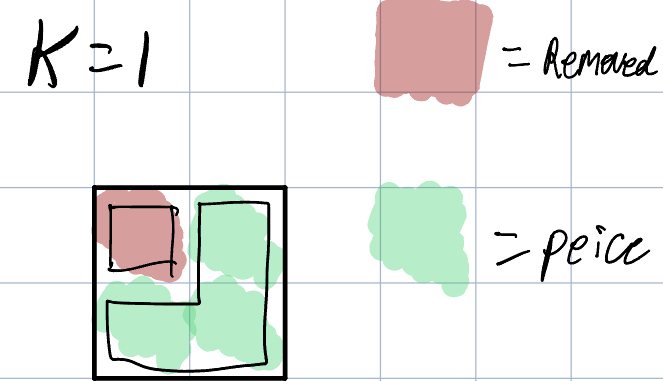
\includegraphics[width=0.5\textwidth]{images/1.1.jpeg}
\end{center}
We can use this as a base case for our
divide and conquer algorithm. We can now move onto if k is greater than 1.
We move onto if k is equal to 2 which equates to $2^2\times2^2=16$ squares. We can first split the board into 4 equal
squares with the top left square removed with each 2x2 square having only 
4 squares execpt for the top left square. We can now see that we can split this 
into smaller subproblems of size 2x2 from the base case. We can simulate a piece
being removed from the corner by putting a L-shaped piece in the middle of the 
board. We can now fill the board with the corresponding piece for each subproblem
as there is only one possible placement. 
\begin{center}
    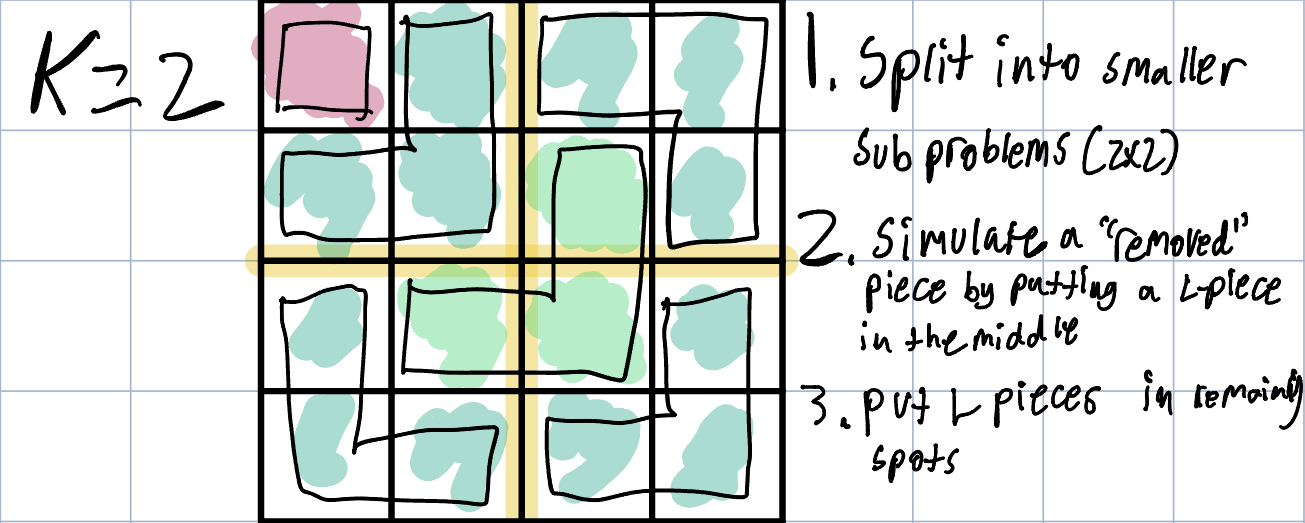
\includegraphics[width=0.5\textwidth]{images/1.2.jpeg}
\end{center}
We can move onto if k is equal to 3 which equates to $2^3\times2^3=64$ squares. We can do the same
process as before by splitting the board into 4 equal squares with the top left square removed leaving
behind 4 4x4 squares (with one of them missing a square).
We can now see that we can split this into even smaller subproblems of size 2x2 which
we can see if the base case. We now can put a L-shaped piece in the middle of each time
we split to simulate a piece being removed from the corner for each 4x4 and 2x2 square.
For the 4x4 squares however the oreintation of the L-shaped piece is different as the middle 
piece that simulates the removed square is in a different position. This however is not a problem
as we can just rotate the piece to fit the square. We can now fill the board with the corresponding
piece for each subproblem which we found from the previous problem.
\begin{center}
    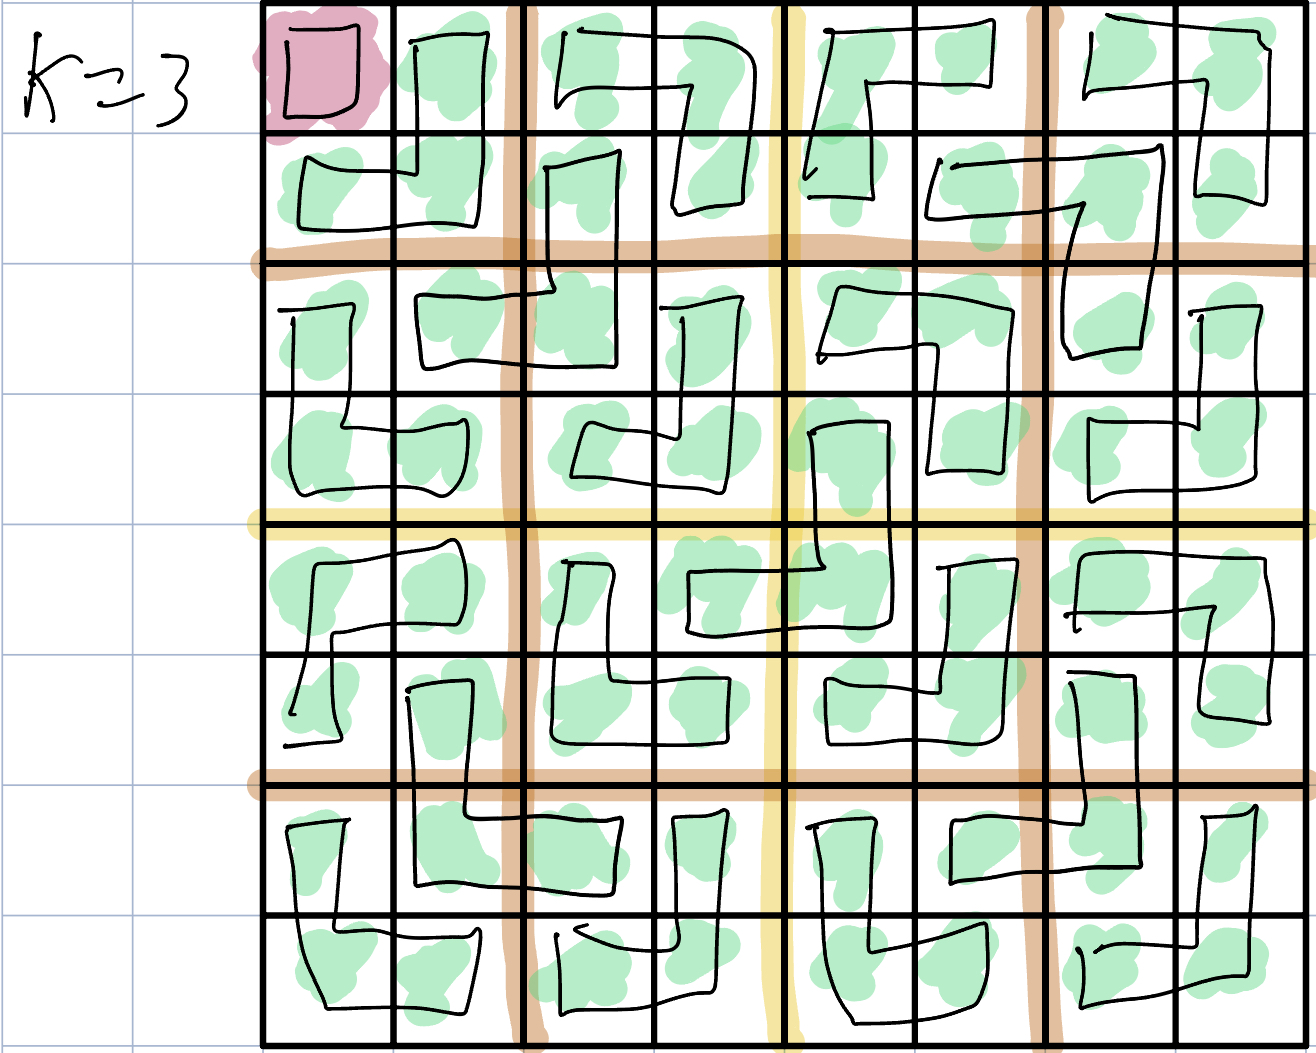
\includegraphics[width=0.5\textwidth]{images/1.3.jpeg}
\end{center}
From all these examples we can derive a pattern that we can use to solve this problem. We split the board into smaller and smaller subproblems until we reach the base.
We can then fill the board with the corresponding piece for each subproblem. From this we can see that this
pattern works for all $k$ as we can just keep splitting the board into smaller and smaller subproblems
until we reach the base case. This means that we can solve this problem by using a divide and conquer
algorithm of splitting the board up. The algorithm is as follows:
\begin{enumerate}
    \item Remove the top left square from the board.
    \item Split the board into 4 equal squares.
    \item For each time you split the board, put a L-shaped piece in the middle of that board.
    \item Repeat steps 2 and 3 until you reach the base case of a 2x2 board for each subproblem.
    \item Fill the board with the corresponding piece for each subproblem.
\end{enumerate}
This algorithm is correct because we are just creating smaller and smaller subproblems that 
simulate the base case of a 2x2 board. This algorithm would have a time complexity of $O(n^2)$
because as we split the board we have to fill the board with a time complexity of $O(n^2)$ for each
subproblem. This means that the total time complexity is $O(n^2)$.

\begin{lstlisting}[language=Python]
# Create a 2^k x 2^k board
k = int(input('Enter a value for k: '))
board = [[0 for _ in range(2**k)] for _ in range(2**k)]

# remove the top left corner square
board[0][0] = -1

def fill_board(board, i, j, size):
    # base case
    # if the size of the board is 2x2, place the L-shaped pieces
    if size == 2:
        # place the L-shaped pieces in remaining squares
        return

    # place L-shaped piece in the middle of the board
    board[i+size//2][j+size//2] = 1
    board[i+size//2-1][j+size//2] = 1
    board[i+size//2-1][j+size//2-1] = 1

    # recursively solve the problem for each quadrant
    fill_board(board, i, j, size//2)
    fill_board(board, i+size//2, j, size//2)
    fill_board(board, i, j+size//2, size//2)
    fill_board(board, i+size//2, j+size//2, size//2)

fill_board(board, 0, 0, 2**k)

\end{lstlisting}


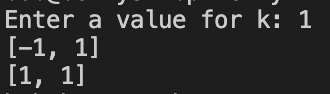
\includegraphics[width=0.3\textwidth]{images/1.code1.png}
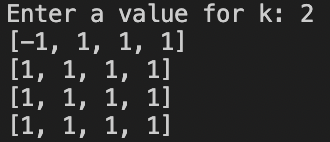
\includegraphics[width=0.3\textwidth]{images/1.code2.png}
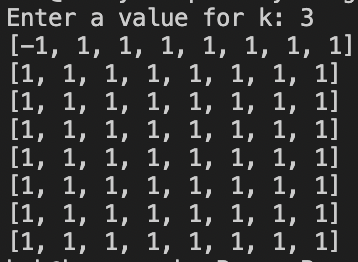
\includegraphics[width=0.3\textwidth]{images/1.code3.png}


\pagebreak

\section*{Problem 2}

You are given an unsorted list $L$ that has $k \ge 0$ pairs of indices $i < j$ such that $L[i] > L[j]$.
These are called $inverted$ $pairs$. Develop an $O(n log n)$ algorithm that counts the number of
inverted pairs (i.e. compute the value $k$).

We can solve this problem with a well known algorithm called merge sort.
Merge sort can be used to sort a list in $O(n log n)$ time. We can use this
algorithm to count the number of inverted pairs. We can first split the list
into multiple sublists of size 1. We can then merge the sublists together in
order. If we merge two sublists together, we can count the number of inverted
pairs per merge. Each merge would create a list that we can go through and count
the number of inverted pairs. After we merge that layer of sublists, we can
merge the next layer of sublists. We can repeat this process until we have
merged all the sublists together. This means that we can count the number of
inverted pairs in $O(n log n)$ time. The algorithm is as follows:
\begin{enumerate}
    \item Split the list into sublists of size 1.
    \item Merge the sublists together in order.
    \item Iterate through each list and count the number of inverted pairs per merge.
    \item Repeat steps 2 and 3 until we have merged all the sublists together.
\end{enumerate}

The time complexity of this algorithm is $O(n log n)$ because we are splitting the list into sublists
of size 1 and then merging the sublists together in order. This means that we are splitting the list
into sublists of size 1 in $O(n)$ time and then merging the sublists together in order in $O(n log n)$
time. This means that the total time complexity is $O(n log n)$.

\pagebreak

\section*{Problem 3}
The \textit{best subset problem} is defined as, given a list $(x_1, x_2, \ldots , x_n)$ of integers 
(which can be positive, negative, or zero), find $(i, j)$ such that $x_i + x_{i+1} + \ldots + x_j$ is 
maximum for any $1 \leq i \leq j \leq n.$ For example, if $n = 10$ and the input is $(4, -8, -5, 8, -4, 3, 6, -3, 2, -11)$ 
then the output is $x_4 + x_5 + x_6 + x_7 = 8 - 4 + 3 + 6 = 13.$

\begin{enumerate}
    \item{Develop an $O(n)$ algorithm for the related problem, \textit{best subset middle} or BSM. The input to BSM is a list $(x_1, x_2, \ldots , x_n)$ of integers (which can be positive, negative, or zero) and the output is the maximum value of $x_i + x_{i+1} + \ldots + x_j$ such that $[i, j]$ spans $\frac{n}{2}$, in other words, for all possibilities for $i$ and $j$ such that $1 \leq i \leq \frac{n}{2} \leq j \leq n.$}
    \item{Design a recursive algorithm for the best subset problem with runtime $O(n log n)$ that
    uses the BSM function.}
    \item{Argue that your algorithm is indeed correct and prove the runtime is $O(n log n).$}
    \item{ (Extra credit: 5pts) Design an algorithm for the best subset problem that has $O(n)$
    runtime. Argue why your algorithm is correct and has $O(n)$ runtime.}
\end{enumerate}

\textbf{Solution:}
\begin{enumerate}
    \item We can create a O(n) algorithm for the best subset middle problem by splitting the list into two sublists. 
    We can then find the maximum value of the first sublist and the maximum value of the second sublist using pointers.
    As we iterate through each sublist, we can keep track of the maximum value and the index of the maximum value for each sublist.
    We can then add the maximum value of the first sublist and the maximum value of the second sublist to find the maximum value of the
    first sublist and the second sublist combined. We are basically finding the maximum value of the first sublist and the maximum value of the second sublist
    from the middle of the list. If we find a value that is greater than the maximum value of the first sublist and the maximum value of the second sublist combined,
    we can update the maximum value of the first sublist and the maximum value of the second sublist combined. We can repeat this process until we have iterated
    through the entire list. This means that we can find the maximum value of the first sublist and the maximum value of the second sublist combined in $O(n)$ time.
    \item We can design a recursive algorithm for the best subset problem with runtime $O(n log n)$ that uses the BSM function. 
    Since we have already created an algorithm for the BSM problem that has runtime $O(n)$, we can use this algorithm to solve the best subset problem.
    We can format this like a divide and conquer algorithm. We can keep splitting the list into two sublists until we have a list of size 1.
    We can then merge the sublists together in order. Each merge would create a list that we can go through and find the maximum value of the sublist.
    After we merge that layer of sublists, we can merge the next layer of sublists, if that layer has a greater value than the previous layer then 
    we can update the maximum value of the sublist. We can repeat this process until we have merged all the sublists together. This means that we can find the maximum value of the sublist in $O(n log n)$ time
    as we are iterating through each sublist with a runtime of $O(n)$ and then merging the sublists together in order in $O(n log n)$ time.
    \item We can prove that our algorithm is indeed correct and prove the runtime is $O(n log n)$. We can prove that our algorithm is correct by
    showing that the algorithm is a divide and conquer algorithm, and behaves similarly to merge sort. We split the problem into subproblems,
    of smaller lists of size 1. By splitting the problem into subproblems, there are going to be $O(log n)$ subproblems. 
    At each level there is going to be $O(n)$ work to do. This means that with each level along with the total amount of levels,
    we are going to have $O(n log n)$ work to do. This means that the runtime is $O(n log n)$.
    \item We can design an algorithm for the best subset problem that has $O(n)$ runtime. We can use a algorithm called
    Kadane's algorithm to solve this problem. We can iterate through the list and keep track of a current maximum value and a global maximum value.
    We can then update the current maximum value by adding the current value to the current maximum value. If the current maximum value is less than the current value,
    we can update the current maximum value to the current value. We can then update the global maximum value by comparing the current maximum value to the global maximum value.
    We can repeat this process until we have iterated through the entire list. This means that we can find the maximum value of the sublist in $O(n)$ time.



\end{enumerate}

\end{document}
